\chapter*{Anhang} \fancyhead[RE,RO]{}
Auswertung der Testreihe: Vergleich Inductive Visual Miner und Interactive Data-aware Heuristics Miner
\captionsetup[table]{list=no}
\captionsetup[figure]{list=no}
\subsubsection{Ergebnisse der Versuchsreihe}\label{results}
\begin{figure}[!ht]
    \centering
    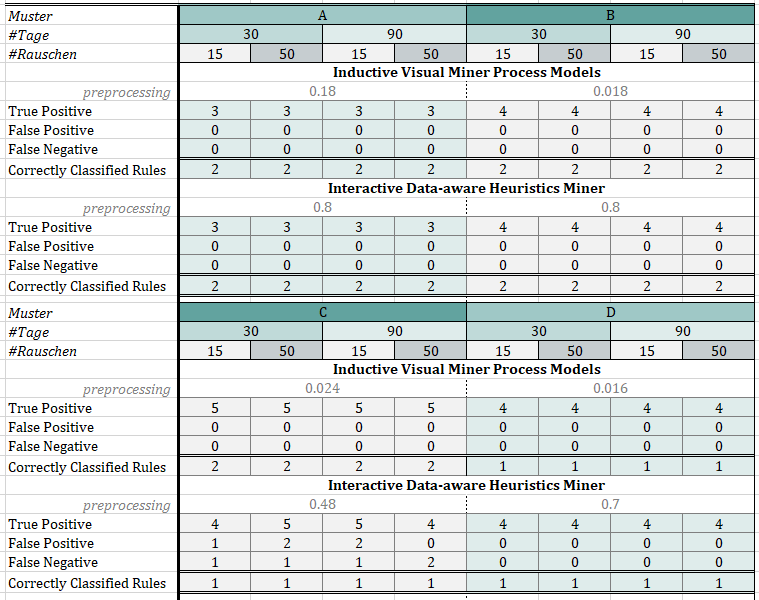
\includegraphics[width=0.9\textwidth]{figures/Appbildungen/tab1.PNG}
    \caption{Ergebnisse Versuchsreihe 'A' - 'D' des Inductive und Heuristic Miners}
    \label{tab1}
\end{figure}

\begin{figure}[!ht]
    \centering
    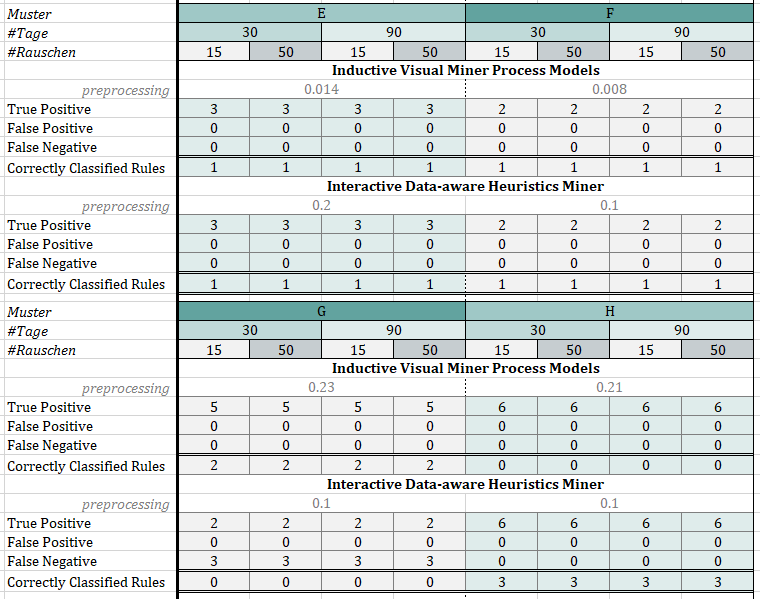
\includegraphics[width=\textwidth]{figures/Appbildungen/tab2.PNG}
    \caption{Ergebnisse Versuchsreihe 'E' - 'H' des Inductive und Heuristic Miners}
    \label{tab2}
\end{figure}

\begin{figure}[!ht]
    \centering
    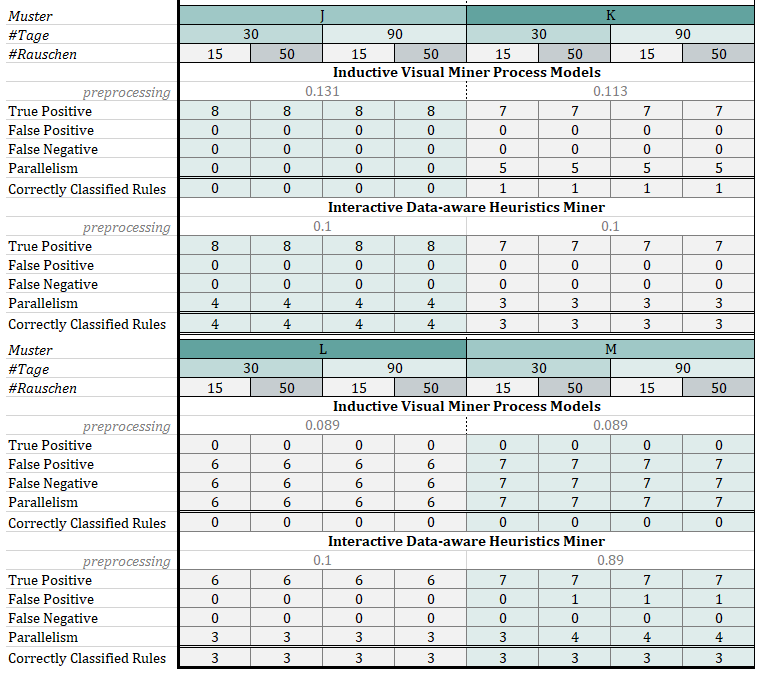
\includegraphics[width=\textwidth]{figures/Appbildungen/tab3.PNG}
    \caption{Ergebnisse Versuchsreihe 'J' - 'M' des Inductive und Heuristic Miners}
    \label{tab3}
\end{figure}

\clearpage
\subsubsection{Eventlogs generieren}\label{lst:generate}
\small
\begin{lstlisting}[language=Python]
import csv
import time
import random
import datetime as dt
from datetime import timedelta
#...
def addnoise(noise, casename, currenttimestamp):
    totalseconds_in_range = 5 * 60 * 60
    noisesum = int(( float(noise) / float(100.) ) * len(pattern_a)+len(pattern_b))
    for i in range(noise):
        timestamp_noise_entry = currenttimestamp +dt.timedelta(seconds=random.randint(0,totalseconds_in_range))
        randNoiseEntrance = random.randint(0,(len(pattern_n)-1))
        eventlog.append([casename, str(timestamp_noise_entry), pattern_n[randNoiseEntrance][0],  pattern_n[randNoiseEntrance][0]+" "+pattern_n[randNoiseEntrance][1]])
        
def eventlogfill():
    var_case = 'A'
    var_case_ext = 'A'
    v = var_case_ext+var_case
    for i in range(days):
        minutes_diff = 30
        timestamp_it = timestamp_start + dt.timedelta(days=i)
        timestamp_it_end = timestamp_it + dt.timedelta(hours=5)
        totalseconds_in_range = 5 * 60 * 60
        
        addnoise(noise, v,timestamp_it)
        randsec = random.randint(5,55)
    
        if (i) % 10 == 0:
            #i
            timestamp_it_one = timestamp_it + dt.timedelta(minutes=(minutes_diff))
            eventlog.append([str(v), str(timestamp_it_one), rule_X_i[0],  
                                        rule_X_i[1]])
            timestamp_it_one_b = timestamp_it_one+ dt.timedelta(seconds=80+3*randsec)
            eventlog.append([str(v), str(timestamp_it_one_b),  rule_X_ii[0],  
                                        rule_X_ii[1]])
            #ii
            timestamp_it_two = timestamp_it_one_b + dt.timedelta(minutes=(minutes_diff))            
            eventlog.append([str(v), str(timestamp_it_two), rule_Y_i[0],  
                                       rule_Y_i[1]])
            timestamp_it_two_b = timestamp_it_two+ dt.timedelta(seconds=80+3*randsec)        
            eventlog.append([str(v), str(timestamp_it_two_b), rule_Y_ii[0],  
                                        rule_Y_ii[1]])
            #iii
            timestamp_it_three = timestamp_it_two_b + dt.timedelta(minutes=(minutes_diff))        
            eventlog.append([str(v), str(timestamp_it_three),  rule_Z_i[0],  
                                        rule_Z_i[1]])
            timestamp_it_three_b = timestamp_it_three+ dt.timedelta(seconds=80+3*randsec)
            eventlog.append([str(v), str(timestamp_it_three_b),  rule_Z_ii[0],  
                                        rule_Z_ii[1]])
            timestamp_it_three_c = timestamp_it_three_b+ dt.timedelta(seconds=80+3*randsec)
            eventlog.append([str(v), str(timestamp_it_three_c),  rule_Z_iii[0],  
                                        rule_Z_iii[1]])
        #...
        v = var_case_ext+var_case+""
        
        if ord(var_case)>=90:
            var_case = 'A'
            var_case_ext = chr(ord(var_case_ext) + 1)
        else:
            var_case = chr(ord(var_case) + 1)
    eventlog.sort(key=lambda events: events[1])

def createcsv():
    with open('...\\CSVtoXES\\NAME\\IN\\'+filename+'.csv', 'w', newline='') as csvfile:
            filewriter = csv.writer(csvfile, delimiter=',', quotechar='|', quoting=csv.QUOTE_MINIMAL)
            filewriter.writerow(['case', 'timestamp', 'resource', 'activity'])
            for i in range(len(eventlog)):
                filewriter.writerow(eventlog[i])
    print("writing completed")

eventlogfill()
createcsv()
\end{lstlisting}

\clearpage
\subsubsection{Eventlogs nach XES Parsen}
\begin{lstlisting}[language=Python]
def generateXes(NDUI):
    records = []
    f = open(OUTdirectory+NDUI+".xes", "w+")
  
    iterlines = iter(csvfile)
    next(iterlines)
    for line in csvfile:
        parts = line.split(',')
        case = parts[0]
        timestamp = parts[1]
        resource = parts[2]
        activity = parts[3].rstrip()
    
        datetime_object = datetime.strptime(timestamp, '%Y-%m-%d %H:%M:%S')
    
        record = {"case":case, "timestamp":datetime_object, "resource":resource, "activity":activity}
        records.append(record)
    csvfile.close()
    
    header = """<?xml version="1.0" encoding="UTF-8" ?>
    <!-- This file has been generated with the OpenXES library. It conforms -->
    <!-- to the XML serialization of the XES standard for log storage and -->
    <!-- management. -->
    <!-- XES standard version: 1.0 -->
    <!-- OpenXES library version: 1.0RC7 -->
    <!-- OpenXES is available from http://www.openxes.org/ -->
    <log xes.version="1.0" xes.features="nested-attributes" openxes.version="1.0RC7">
    	<extension name="Lifecycle" prefix="lifecycle" uri="http://www.xes-standard.org/lifecycle.xesext"/>
    	<extension name="Time" prefix="time" uri="http://www.xes-standard.org/time.xesext"/>
    	<extension name="Concept" prefix="concept" uri="http://www.xes-standard.org/concept.xesext"/>
    	<classifier name="Event Name" keys="concept:name"/>
    	<classifier name="(Event Name AND Lifecycle transition)" keys="concept:name lifecycle:transition"/>
    	<string key="concept:name" value="XES Event Log"/>"""
    footer = "</log>"
    
    f.write(header)
    currentday=None
    currentmonth=None
    currentyear=None
    id = 100
    for record in records:
        if currentday is None:
            f.write('\t<trace>\n')
            currentday = record['timestamp'].day
            currentmonth= record['timestamp'].month
            currentyear= record['timestamp'].year
            case = record['case']
            print(str(case))
            f.write('\t\t<string key="concept:name" value="'+case+'"/>\n')
        else:
            if currentday != record['timestamp'].day or currentmonth != record['timestamp'].month or currentyear != record['timestamp'].year:
                f.write('\t</trace>\n')
                f.write('\t<trace>\n')
                case = record['case']
                print(str(case))
                f.write('\t\t<string key="concept:name" value="'+case+'"/>\n')
                #case = chr(ord(case)+1)
                currentday = record['timestamp'].day
                currentmonth= record['timestamp'].month
                currentyear= record['timestamp'].year
        f.write('\t\t<event>\n')
        f.write('\t\t\t<string key="resource" value="'+record['resource']+'"/>\n')
        f.write('\t\t\t<string key="lifecycle:transition" value="start"/>\n')
        f.write('\t\t\t<string key="concept:name" value="'+record['activity']+'"/>\n')
        datestring = record['timestamp'].strftime('%Y-%m-%dT%H:%M:%S.000+02:00')
        f.write('\t\t\t<date key="time:timestamp" value="'+datestring+'"/>\n')
        f.write('\t\t\t<int key="Event ID" value="'+str(id)+'"/>\n')
        id +=1
        f.write('\t\t</event>\n')
    
    f.write('\t</trace>')    
    f.write(footer)

for filename in os.listdir(directory):
    if(filename.endswith('.csv')):
        csvfile=open(os.path.join(directory, filename), 'r')
        print(filename)
        generateXes(filename)
    else:
        continue

\end{lstlisting}

\clearpage
\subsubsection{Konfiguration der Versuchsreihen}\label{sec:config}
Eingabedaten für den Eventloggenerator.
Je Versuchsreihe wurden vier Eventlogs generiert, die jeweils Zeilen der Schemata 'A' - 'M' enthielten.
\begin{table}[!ht]
\centering
\resizebox*{!}{0.8\textheight}{%
\begin{tabular}{llll}
\hline
\textbf{Bez.} & \textbf{Resource}             & \textbf{Activity}                         & \textbf{About}            \\ \hline
A             & \textit{}                     & \textit{}                                 & Rules                     \\
i             & \textit{Doorbell}             & \textit{ringing}                          & \multicolumn{1}{r}{2}     \\
ii            & \textit{Coffee Maker}         & \textit{turned to ON}                     & Nodes                     \\
              & \textit{Coffee Maker}         & \textit{Two Esprosso Cups}                & \multicolumn{1}{r}{3}     \\ \hline
B             & \textit{}                     & \textit{}                                 & Rules                     \\
i             & \textit{Coffee Maker}         & \textit{turned to ON}                     & \multicolumn{1}{r}{2}     \\
              & \textit{Coffee Maker}         & \textit{Two Esprosso Cups}                & Nodes                     \\
ii            & \textit{Doorbell}             & \textit{recognized a face (registered)}   & \multicolumn{1}{r}{4}     \\
              & \textit{Doorbell}             & \textit{ringing}                          &                           \\ \hline
C             & \textit{}                     & \textit{}                                 & Rules                     \\
i             & \textit{Alarm}                & \textit{turned on}                        & \multicolumn{1}{r}{2}     \\
              & \textit{Bathroom Light}       & \textit{set to ON}                        & Nodes                     \\
              & \textit{Bathroom Light}       & \textit{set to OFF}                       & \multicolumn{1}{r}{5}     \\
ii            & \textit{Coffee Maker}         & \textit{Two Esprosso Cups}                &                           \\
              & \textit{Coffee Maker}         & \textit{set to OFF}                       &                           \\ \hline
D             & \textit{}                     & \textit{}                                 & Rules                     \\
i             & \textit{Garage Door}          & \textit{Garage Door opened}               & \multicolumn{1}{r}{1}     \\
              & \textit{Garage Door}          & \textit{Garage Door closed}               & Nodes                     \\
              & \textit{smartlight 02}        & \textit{switched to ON}                   & \multicolumn{1}{r}{4}     \\
              & \textit{smartlight 02}        & \textit{switched to OFF}                  &                           \\ \hline
E             & \textit{}                     & \textit{}                                 & Rules                     \\
i             & \textit{smartlight main}      & \textit{turned to ON}                     & \multicolumn{1}{r}{1}     \\
              & \textit{weather sensor}       & \textit{currently snowing}                & Nodes                     \\
              & \textit{heating element}      & \textit{turned to ON}                     & \multicolumn{1}{r}{3}     \\ \hline
F             & \textit{}                     & \textit{}                                 & Rules                     \\
i             & \textit{front door}           & \textit{unlocked}                         & \multicolumn{1}{r}{1}     \\
              & \textit{smartlight 02}        & \textit{turned to on}                     & Nodes                   2 \\ \hline
G             & \textit{}                     & \textit{}                                 & Rules                     \\
i             & \textit{Garage Door}          & \textit{opened}                           & \multicolumn{1}{r}{2}     \\
              & \textit{Garage Door}          & \textit{closed}                           & Nodes                     \\
              & \textit{smartlight 02}        & \textit{switched to ON}                   & \multicolumn{1}{r}{7}     \\
              & \textit{smartlight 02}        & \textit{switched to OFF}                  &                           \\
ii            & \textit{Alarm}                & \textit{turned on}                        &                           \\
              & \textit{Bathroom Light}       & \textit{set to ON}                        &                           \\
              & \textit{Bathroom Light}       & \textit{set to OFF}                       &                           \\ \hline

\end{tabular}%
}
\caption{Konfiguration Versuchsreihe 'A' - 'G'}
\label{tab:Versuchskonfig1}
\end{table}

\clearpage
\begin{table}[]
\centering
\resizebox{\textwidth}{!}{%
\begin{tabular}{llll}
\hline
\textbf{Bez.} & \textbf{Resource}             & \textbf{Activity}                         & \textbf{About}            \\ \hline
H             & \textit{}                     & \textit{}                                 & Rules                     \\
i             & \textit{Smart TV}             & \textit{turned to ON}                     & \multicolumn{1}{r}{3}     \\
              & \textit{Smart TV}             & \textit{switched to CHANNEL 1}            & Nodes                     \\
ii            & \textit{Smart Alarm Clock}    & \textit{turned to ON}                     & \multicolumn{1}{r}{6}     \\
              & \textit{CLEVER Coffee Maker}  & \textit{two Espresso Cups}                &                           \\
iii           & \textit{Nested Thermostat}    & \textit{SET TO 18 DEG}                    &                           \\
              & \textit{Light Fixture}        & \textit{turned to ON}                     &                           \\ \hline
J             & \textit{}                     & \textit{}                                 & Rules                     \\
i             & \textit{Smart TV}             & \textit{turned to ON}                     & \multicolumn{1}{r}{4}     \\
              & \textit{Smart TV}             & \textit{switched to CHANNEL 1}            & Nodes                     \\
ii            & \textit{Smart Alarm Clock}    & \textit{turned to ON}                     & \multicolumn{1}{r}{8}     \\
              & \textit{CLEVER Coffee Maker}  & \textit{two Espresso Cups}                &                           \\
iii           & \textit{Nested Thermostat}    & \textit{SET TO 18 DEG}                    &                           \\
              & \textit{Light Fixture}        & \textit{turned to ON}                     &                           \\
iv            & \textit{Light Fixture}        & \textit{turned to OFF}                    &                           \\
              & \textit{Nested Thermostat}    & \textit{SET TO 13 DEG}                    &                           \\ \hline
K             & \textit{}                     & \textit{}                                 & Rules                     \\
i             & \textit{Smart TV}             & \textit{turned to ON}                     & \multicolumn{1}{r}{3}     \\
              & \textit{Smart TV}             & \textit{switched to CHANNEL 1}            & Nodes                     \\
              & \textit{Smart TV}             & \textit{set Volume to 22}                 & \multicolumn{1}{r}{7}     \\
ii            & \textit{Smart Alarm Clock}    & \textit{turned to ON}                     &                           \\
              & \textit{CLEVER Coffee Maker}  & \textit{two Espresso Cups}                &                           \\
iii           & \textit{Nested Thermostat}    & \textit{SET TO 18 DEG}                    &                           \\
              & \textit{Light Fixture}        & \textit{turned to ON}                     &                           \\ \hline
L*            & \textit{}                     & \textit{}                                 & Rules                     \\
i             & \textit{Smart TV}             & \textit{turned to ON}                     & \multicolumn{1}{r}{3}     \\
              & \textit{Smart TV}             & \textit{switched to Streaming Service TM} & Nodes                     \\
ii            & \textit{Smart Alarm Clock}    & \textit{turned to ON}                     & \multicolumn{1}{r}{6}     \\
              & \textit{CLEVER Coffee Maker}  & \textit{two Espresso Cups}                &                           \\
iii           & \textit{Garage Door}          & \textit{Light turned Off}                 & *every other day          \\
              & \textit{Garage Door}          & \textit{Door closed}                      &                           \\ \hline
M*            & \textit{}                     & \textit{}                                 & Rules                     \\
i             & \textit{Smart TV}             & \textit{turned to ON}                     & \multicolumn{1}{r}{3}     \\
              & \textit{Smart TV}             & \textit{switched to Streaming Service TM} & Nodes                     \\
ii            & \textit{Garage Door}          & \textit{Light turned Off}                 & \multicolumn{1}{r}{7}     \\
              & \textit{Garage Door}          & \textit{Door closed}                      &                           \\
iii           & \textit{Nested Thermostat}    & \textit{SET TO 16 DEG}                    & *every third day          \\
              & \textit{Main Light}           & \textit{turned to OFF}                    &                           \\
              & \textit{Floor Heating System} & \textit{turned to OFF}                    &                           \\ \hline
			  \end{tabular}%
}
\caption{Konfiguration Versuchsreihe 'H' - 'M'}
\label{tab:Versuchskonfig2}
\end{table}



\clearpage
\subsubsection{Clientseitige Regelverarbeitung}\small
\begin{lstlisting}[language=Java]
public class PMFirebaseMessagingService extends FirebaseMessagingService {

    static String TAG = "ProcessMining MessagingService";
    static String currentToken = "";

    /**
     * Called if InstanceID token is updated. This may occur if the security of
     * the previous token had been compromised. Note that this is called when the InstanceID token
     * is initially generated so this is where you would retrieve the token.
     */
    @Override
    public void onNewToken(String token)
    {
        Log.d(TAG, "Refreshed token: " + token);

        // If you want to send messages to this application instance or
        // manage this apps subscriptions on the server side, send the
        // Instance ID token to your app server.
        currentToken = token;
    }

    public static void refreshID()
    {
        FirebaseInstanceId.getInstance().getInstanceId()
                .addOnCompleteListener(new OnCompleteListener<InstanceIdResult>() {
                    @Override
                    public void onComplete(@NonNull Task<InstanceIdResult> task) {
                        if (!task.isSuccessful()) {
                            //To do//
                            return;
                        }
                        // Get the Instance ID token//
                        String token = task.getResult().getToken();
                        PMFirebaseMessagingService.currentToken = token;
                        Log.d(TAG, "Got Firebase ID: " + token);
                    }
                });

        FirebaseMessaging.getInstance().subscribeToTopic("rules")
                .addOnCompleteListener(new OnCompleteListener<Void>() {
                    @Override
                    public void onComplete(@NonNull Task<Void> task) {

                        if (!task.isSuccessful()) {
                            Log.d(TAG, "Sub to topic not success");
                        }
                        Log.d(TAG, "Sub to topic success");
                    }
                });
    }

    @Override
    public void onMessageReceived(RemoteMessage remoteMessage)
    {
        super.onMessageReceived(remoteMessage);
        String newRules = "";
        for(String key : remoteMessage.getData().keySet())
            Log.d(TAG, "onMessageReceived: got key: " + key);

        if(remoteMessage.getData().containsKey("newRules"))
            newRules = remoteMessage.getData().get("newRules");

        Log.d("onMessreceived","got a message: "+newRules);
        PowerManager pm = (PowerManager) this.getSystemService(Context.POWER_SERVICE);
        boolean isScreenOn = pm.isScreenOn();
        Log.e("screen on.................................", "" + isScreenOn);
        if (isScreenOn == false)
        {
            @SuppressLint("InvalidWakeLockTag") PowerManager.WakeLock wl = pm.newWakeLock(PowerManager.FULL_WAKE_LOCK | PowerManager.ACQUIRE_CAUSES_WAKEUP | PowerManager.ON_AFTER_RELEASE, "MyLock");
            wl.acquire(10000);
            @SuppressLint("InvalidWakeLockTag") PowerManager.WakeLock wl_cpu = pm.newWakeLock(PowerManager.PARTIAL_WAKE_LOCK, "MyCpuLock");

            wl_cpu.acquire(10000);

        }
           startActivity(new Intent(this, MainActivity.class));

        Log.d(TAG, "onMessageReceived: " + remoteMessage.getData().get("message") + " to: " + remoteMessage.getTo());

        Intent intent = new Intent(this, PMRulesTabs.class);
        intent.addFlags(Intent.FLAG_ACTIVITY_CLEAR_TOP);
        PendingIntent pendingIntent = PendingIntent.getActivity(this, 0, intent, PendingIntent.FLAG_ONE_SHOT);

        String channelId = "Default";
        NotificationCompat.Builder builder = new  NotificationCompat.Builder(this, channelId)
                .setSmallIcon(R.mipmap.ic_launcher)
                .setContentTitle("PM")
                .setContentText("new suggested rule received!").setAutoCancel(true).setContentIntent(pendingIntent);;
        NotificationManager manager = (NotificationManager) getSystemService(NOTIFICATION_SERVICE);
        if (Build.VERSION.SDK_INT >= Build.VERSION_CODES.O) {
            NotificationChannel channel = new NotificationChannel(channelId, "Default channel", NotificationManager.IMPORTANCE_HIGH);
            manager.createNotificationChannel(channel);
        }
        manager.notify(0, builder.build());

        try {
            parseReceivedRule(newRules);
        } catch (JSONException e) {
            e.printStackTrace();
        }
    }

    private void parseReceivedRule(String newRule) throws JSONException {
        JSONArray allNodes = new JSONArray(newRule);
        Log.d("process", "All Rules: "+allNodes.getJSONArray(0)+ " 1: "+allNodes.getJSONArray(1));
        for (int i = 0; i < allNodes.length(); i++) {
            try {
                // JSONObject node = rules.getJSONObject(i);
                JSONArray rule = allNodes.getJSONArray(i);
                Log.d("process", "rule: "+i+". "+rule);
                PMRule.processRule(rule);
            } catch (JSONException e) {
                Log.d("process", "Json exception: "+e);
            }
        }
    }
\end{lstlisting}
\normalsize
